\documentclass[12pt, titlepage]{article}

\usepackage{booktabs}
\usepackage{tabularx}
\usepackage{hyperref}
\hypersetup{
    colorlinks,
    citecolor=black,
    filecolor=black,
    linkcolor=red,
    urlcolor=blue
}
\usepackage[round]{natbib}
\usepackage{graphicx}
\graphicspath{ {./Figures/} }
\usepackage{placeins}
\usepackage[block=ragged]{biblatex}
\addbibresource{reference.bib}


\title{SE 3XA3: Software Requirements Specification\cite{website:doc-template}}

\author{Team L03G09
		\\ Qiang Gao gaoq20
		\\ Zhiwei Li liz342
		\\ Longwei Ye yel16
}

\date{\today}



\begin{document}


\maketitle


\pagenumbering{roman}
\tableofcontents
\listoftables
\listoffigures

\begin{table}[!htbp]
\caption{\bf Revision History}
\begin{tabularx}{\textwidth}{p{3cm}p{2cm}X}
\toprule {\bf Date} & {\bf Version} & {\bf Notes}\\
\midrule
2022/2/9  & 1.0   & Complete Section 1\\
2022/2/10 & 1.1   & Complete Section 3\\
2022/2/10 & 1.1.1 & Complete Section 4\\
2022/2/11 & 1.2   & Complete Section 2 and Revise\\
\bottomrule
\end{tabularx}
\end{table}

\newpage

\pagenumbering{arabic}

%This document describes the requirements for ....  The template for the Software
%Requirements Specification (SRS) is a subset of the Volere
%template~\citep{RobertsonAndRobertson2012}.  If you make further modifications
%to the template, you should explicity state what modifications were made.
\section{Project Drivers}

\subsection{The Purpose of the Project}
Gaming on a computer is a convenient and effective way for people's daily entertainment, especially when people are trying to relax themselves. 
We, as the game developers, are trying to provide a satisfying gaming experience for the users by ensuring the quality of the in-game graphic interface as well as the playability of the game itself. The game we are trying to modify is already a classic game. However, we are modifying the project with a modernized and attractive user interface and an enhanced in-game mechanic so that the game can keep track of the latest trends.


\subsection{The Stakeholders}
\subsubsection{The Client}
Project managers who is playing a role as the commissioner and the consultant of the project.

\subsubsection{The Customers}
End users, especially the people who are willing to play games in their spare time.

\subsubsection{Other Stakeholders}
developer, tester, operator

\subsection{Mandated Constraints}
\subsubsection{Schedule Constraints}
We have a project deadline on April 12th, which should be a date we finish
1
 every development, improvement modification, review, test and documentations. 

\subsubsection{Enterprise Constraints}
Since we develop the open-source project on gitlab, there is no limit on players to play the game if they have a browser with JavaScript implemented on their device.

\subsubsection*{Budget Constraints}
N/A

\subsection{Naming Conventions and Terminology}
\begin{table}[!htbp]
\caption{\bf Definitions}
\begin{tabularx}{\textwidth}{p{4cm}p{9cm}X}
\toprule {\bf Terms} & {\bf Definitions}\\
\midrule
JavaScript &  A programming language used to implement core script for World Wide Web.\\
CSS & Cascading Style Sheets, a style sheet language used to describe presentation of the document written in a markin.\\
HTML & The code that is used to structure a web page and its content.\\
GUI & Graphic user interface\\
MVC  & Model-view-controller\\
History & Player score history\\
Single Player Mode & One player playing the game.\\
Double Player Mode & Two players playing against each other.\\
SRS & Software Requirements Specification.\\
Supplement & Food or boosters eaten by the snake to change its velocity or length.\\
End-game Prompt & A prompt with a message "Game Over" appears after the snake dies.\\
\bottomrule
\end{tabularx}
\end{table}

\newpage

\subsection{Relevant Facts and Assumptions}

%User characteristics should go under assumptions.
Since we develop our game on HTML with JavaScript, we assume that our player have a basic browser with JavaScript implemented in their system. 

\section{Functional Requirements}

\subsection{The Scope of the Work and the Product}
Deliverable Deadlines:
    	\begin{itemize}
    		\item Requirements Document Revision 0      (February 11)
    		\item Proof of Concept Demonstration        (Week of February 28)
    		\item Test Plan Revision 0        		    (March 11)
    		\item Design \& Document Revision 0          (March 18)
    		\item Revision 0 Demonstration              (Week of March 21)
    		\item Lab Exercises				            (Throughout Term)
    		\item Final Demonstration (Revision 1)	    (Week of Apr 4)
    		\item Peer Eval of Other Teams Final Demo   (Week of Apr 4)
    		\item Final Documentation				    (April 12)
    	\end{itemize}


\subsubsection{The Context of the Work}
\begin{figure}[!htbp]
    \centering
    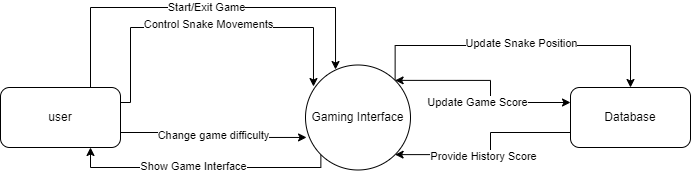
\includegraphics[scale = 0.55]{Figures/context_of_work.png}
    \caption{Work Context Diagram}
\end{figure}

\subsubsection{Work Partitioning}
\begin{table}[!htbp]
\caption{\bf Work Partitioning}
\begin{tabularx}{\textwidth}{p{3cm}p{4cm}p{5.5cm}X}
\toprule {\bf Events} & {\bf Input/Output} & {\bf Description}\\
\midrule
Name the player & A text name(In) & The user names the player for identifying before starting the game.\\
Choose a mode & Mode name(In) & The user chooses a mode (single-player mode or two-player mode) before starting a game.\\
View history & Click history(In) \newline Playing history(Out) & The user views previous playing history including date, scores,name of the player\\
Choose difficulty & Difficulty name(In) & The user chooses the difficulty of the game(Easy, Normal,Difficult).\\
Change snake's direction & Up/down/left/right key(In) & The user changes the direction for the snake moving to.\\

\bottomrule
\end{tabularx}
\end{table}

%\subsubsection{Individual Product Use Cases}

\subsection{Functional Requirements}
\subsubsection{Start the game}
    \begin{itemize}
		\item Requirement number :FR1  
		
		 The user must be able to choose outlook for the snake by choosing different colour before starting the game.
		 
		Rationale: Choosing different outlook for the snake makes the game more interesting and playable.
		
		\item Requirement number :FR2
		
		The user must be able to name the player by typing before starting the game.
		
		Rationale: Name can be used to identify the player and improve penalization, especially useful in two-player mode.
		
		\item Requirement number :FR3
		
		The user must be able to choose mode(single-player mode and two-player mode).
		
		Rationale: There are two modes in the game, one has to be chosen.
		
		\item Requirement number :FR4
		
		The user must be able to view previous playing history including date, scores, name of player.
		
		Rationale: Viewing history helps the user to review their scores and set a goal. 
		
		\item Requirement number :FR5
		
		The user interface must be able to display the rules of the game beside the playing window, both in single-player mode and two-player mode.
		
		Rationale: Displaying rules of the game beside the game window efficiently helps the user know how to play the game.
		
		\item Requirement number :FR6
		
		The user interface must be able to display a short cartoon before starting the game.
		
		Rationale: A short cartoon before starting the game can catch the user's eyes and enhance fun.
		
		\item Requirement number :FR7
		
		The user must be able to choose the difficulty of the game(Easy, Normal, Difficult).
		
		Rationale: Choices for difficulty improve interestingness of the game.
	
	\end{itemize}

\subsubsection{Playing the game}
\begin{itemize}
		\item Requirement number :FR8 
		
		The user interface must refresh the screen at the beginning of the game, updating initial snake position and a random eatable supplement position.  
		 
		Rationale: This should be the starting point for a new turn of the game. We need to ensure that old gaming screen should be refreshed to a new one for this turn.
		
		\item Requirement number :FR9  
		
		 When user press direction keys on the keyboard(Up, Down, Left, Right), except for the direction for snake's body, the heading direction of the snake must be changed to the indicated direction.
		 
		Rationale: This is the way user can control the snake's movement in the game.
		
		\item Requirement number :FR10 
		
		 The user interface must be able to refresh the gaming screen with certain frequency, updating the snake's length and position.
		 
		 Rationale: The current state and position of the snake of the game should be provided to user by refreshing the screen.
		\item Requirement number :FR11  
		
		 After every refreshing, it must be checked that whether the snake's head touches walls or its own body. If so, the game should be ended. 
		 
		Rationale: The basic criteria to end a game should be checked in every snake's move turn. 
		\item Requirement number :FR12  
		
		 After every refreshing, it must be checked that whether the snake's head touches a supplement. If so, the snake's status should be updated as the rule specified. 
		 
		Rationale: This is the checking phase for the snake possible eaten supplement, as eating is an important main part of the game to raise user's goal.
		
	\end{itemize}
\subsubsection{End the game}
\begin{itemize}
		\item Requirement number :FR13  
		
		The screen must be frozen if the game reach an end. 
		 
		Rationale: To inform a game turn's ending to player, we need to freeze the screen to prevent further in-game action.
		\item Requirement number :FR14  
		
		A pop-out information prompt must be displayed to show "Game Over" information with the cumulative game score.
		 
		Rationale: To explicitly inform player the ending of the game, a prompt is needed.
		\item Requirement number :FR15  
		
		The user interface must be able to update the score in history, keep the screen frozen till the player click the new game button
		 
		Rationale: We need to keep the record of the players score and wait for the new game command, otherwise we should not allow player to modify the game or the data.
	\end{itemize}

\subsubsection{During the game: snake eats a booster element}
\begin{itemize}
		\item Requirement number :FR1  
		
		If the eaten supplement is blue, the snake is moving twice faster from now on without adding the length. 2 score is added to the cumulative score.
		 
		Rationale: It is acted as an element in the game rule to raise games' amusement.
		\item Requirement number :FR2  
		
		If the eaten supplement is red, the snake is gaining 3 length in the following 3 refresh turn. 5 score is added to the cumulative score.
		 
		Rationale: It is also acted as an element in the game rule to raise games' amusement.
		\item Requirement number :FR3   
		
    	If the eaten supplement is white, the snake is gaining 1 length in the following 1 refresh turn. 1 score is added to the cumulative score.
		
		Rationale: It is the basic condition for the snake to get a supplement to raise the score.  
		
	\end{itemize}

\section{Non-functional Requirements}

\subsection{Look and Feel Requirements}

\begin{itemize}
\item The user interface should be basically clear to recognize every functionality. 
\item The GUI should look relaxing and amusing, some warm and light color should be mostly used.
\item In the main gaming window, the distinct color should be used to inform different element in the game.

\end{itemize}

\subsection{Usability and Humanity Requirements}
\begin{itemize}
\item The instructions should be clearly declared in the user interface as guidance. 
\item The difficulty of the game should be reasonable for most people, like reaction speed demand and color distinguishing.

\end{itemize}
\subsection{Performance Requirements}

\subsubsection{Capacity Requirements}
The game shall not exceed the memory the machine that is running the game.

\subsection{Operational and Environmental Requirements}
The game should be run on different devices as long as the device has connected to the keyboard hardware and has the web browser application pre-installed.

\subsection{Maintainability and Support Requirements}
\subsubsection{Maintainability Requirements}
The code of the project should have a clear structure for the convenience of further maintains.
\subsubsection{Support Requirements}
Ensure most of the machines(e.g. laptops installed with different operation systems) can run the game.


\subsection{Security Requirements}
\subsubsection{Privacy Requirements}
The game shall not collect any means of user data from the machine that is running the game.

\subsection{Cultural Requirements}
\begin{itemize}
    \item The game should be be offensive to ethnic or religious believes.
    \item The game should provide a English-based interface to the users.
\end{itemize}

\subsection{Legal Requirements}
\begin{itemize}
    \item The game should not violate any laws.
    \item The game should follow the \textit{Apache License 2.0 license.}
\end{itemize}


\subsection{Health and Safety Requirements}
The game should not contain any means of violent contents.

%This section is not in the original Volere template, but health and safety are
%issues that should be considered for every engineering project.

\section{Project Issues}

\subsection{Open Issues}
There is currently no open issues.
\subsection{Off-the-Shelf Solutions}
The modular components from the original SnakeGame project.

\subsection{New Problems}
\subsubsection{Effects on the Current Environment}
The change of the appearance of the GUI will provided the users a modernized look of the game. Besides, the addition of the in-game props will affect the game by increasing the play-ability.

\subsubsection{Effects on the Installed Systems}
The new interface is independent to the old system. In other words, they are not coexisting with each other.


\subsection{Tasks}
The SnakeGame project is delivering under the schedules from \textit{SE 3XA3} outline. The planned final demonstration and documentation of the project will be delivered no later than 
April 12th, 2022. During the developing process, the deliverable stages include:
\begin{itemize}
    \item Problem statement
    \item Development plan
    \item Requirements document Revision 0
    \item Proof of concept demonstration 
    \item Test plan Revision 0
    \item Design \& Document Revision 0
    \item Revision 0 demonstration
    \item Peer evaluation of other teams final demo
    \item Final demonstration \& documentation
\end{itemize}

\subsection{Migration to the New Product}
The original MVC structure can be kept as basics to add new features on. 

\subsection{Risks}
\subsubsection{Technical Risks}
\begin{itemize}
    \item New programming language learning(JavaScript, Html, Css), familiar with the coding environment.
    \item Understanding existing GUI and making some adjustments suitable with the current GUI design.
    \item Testing environment for JavaScript should be chosen carefully since we lack JavaScript testing experience.

\end{itemize}

\subsection{Costs}
No. Because all the resources used are free.
\subsection{User Documentation and Training}
\subsubsection{User Documentation}
N/A
\subsubsection{Training}
A short game instructions is displayed on the user-interface, which includes snake control functions and in-game elements.

\subsection{Waiting Room}
Additional in-game props to enrich the game content, and user-customized features like optional background.

\subsection{Ideas for Solutions}
\begin{itemize}
    \item Supporting documentations for JavaScript, HTML, and CSS.
    \item Current examples(open-source projects) that can be referred.
\end{itemize}

\section{Appendix}
\subsection{Gantt Chart}
Please refer \textit{ProjectSchedule.pdf} at the same folder.

\printbibliography

\end{document}